\chapter{Experiments and Results}
\label{chap:experiments}
This chapter presents a series of experiments designed to answer the research questions posed in \autoref{chap:intro}, focusing on the evaluation of the Mamba-\acrshort{s6} (\acrshort{vms}) model for temporal event spotting in football video. The accuracy and runtime are compared against the \acrshort{tdeed} baseline, I investigate the impact of feature dimensionality, and perform a Bayesian hyperparameter sweep to optimize performance.


\section{Experiment 1: Compare accuracy between \acrshort{tdeed} and mamba}
\label{sec:experiment1}
The first experiment compares accuracy from \acrfull{tdeed} and \acrfull{vms}. The goal is to determine if the \acrshort{vms} model can achieve similar or better accuracy than the \acrshort{tdeed} model. The models are trained on the SoccerNet-V2 dataset \cite{deliege_soccernet-v2_dataset_2021}. They are evaluated using mean average precision (\acrshort{map}) and \acrshort{map}@50 metrics.

\subsection{Setup}
\label{ssec:ex1_setup}
We trained three models on the SoccerNet-V2 dataset \cite{deliege_soccernet-v2_dataset_2021}:  
\begin{itemize}
    \item \acrshort{vms}-80\_20 using an 80\%/20\% train/val split,  
    \item \acrshort{vms}-70\_30 using a 70\%/30\% split, and  
    \item \acrshort{tdeed} with four matches for training and one for validation (equivalent to 80\%/20\%).  
\end{itemize}

All models used default hyperparameters from their original papers. Performance was measured by mean \acrfull{map} and \acrshort{map}@50 under a \(\pm 1\) s tolerance window.

\todo{talk about annotation edit? mentioned in method}

\subsection{Results}
\label{ssec:ex1_results}
\begin{table}[ht]
    \centering
    \begin{tabular}{lccc}
        \toprule
        Model & average \acrshort{map} (\%)  & validation \acrshort{map}@50 (\%) & test \acrshort{map}@50 (\%)\\
        \midrule
        \acrshort{tdeed} &  \textemdash & 20.78 & \textbf{47.65}\\
        \acrshort{vms} (Mamba-\acrshort{s6})   &  \textbf{45.99}   & 43.62 & \textemdash \\
        % \acrshort{vms}-70\_30 (Mamba-\acrshort{s6})   & 48.73 & 46.46 \\
        \bottomrule
    \end{tabular}
    \caption{Accuracy comparison on SoccerNet-V2.}
    \label{tab:results_ex1}
\end{table}

The \acrshort{vms} model (Mamba-\acrshort{s6}) had an average \acrshort{map}, achieving \textbf{45.99\%}. The \acrshort{tdeed} model's average \acrshort{map} is not calculated as there is no \acrshort{iou}, but its validation \acrshort{map}@50 was 20.78\%. In the validation \acrshort{map}@50 category, the \acrshort{vms} model significantly outperformed \acrshort{tdeed}, scoring (43.62\%) compared to \acrshort{tdeed}'s (20.78\%).

Conversely, the \acrshort{tdeed} model achieved a higher test \acrshort{map}@50 of \textbf{47.65\%}. Whereas the corresponding test metric for the \acrshort{vms} model is not provided or calculated. There is a significant disparity between \acrshort{tdeed}'s validation and test performance. This is primarily due to differences in stride during prediction, with the validation model using a stride of two, effectively halving its temporal resolution compared to the test evaluation. 

% Furthermore, it is mentioned that \acrshort{tdeed} incorporates significant postprocessing, as illustrated in \autoref{tab:results_ex1}. The discussion also posits that the fine-grained nature of the action spotting task, with its narrow \( \pm 1 \) second tolerance window, is inherently well-suited to the \acrshort{tdeed} model's design.

\subsection{Discussion}
\label{ssec:ex1_discussion}

The large difference in validation \acrshort{map}@50 for \acrshort{tdeed} could be a result of lacking postprocessing. \acrshort{tdeed} uses two different functions for predicting the test \acrshort{map} and the validation \acrshort{map}. The test evaluator applies soft non-maximum suppression to remove redundant detections, while the validation does not remove redundant predictions. In addition to this, the validation predicts with a stride of \(2\), but the test has a stride of \(1\). With \(fps=25\) and a \(tolerance = \pm 1s\), this reduction in temporal resolution hinders the predictions from hitting the tolerance window. 


% \acrshort{vms} does little preprocessing, and its only configurable parameter was the top \(k\) classes to predict in each step. \acrshort{vms} predicts the likelihood of different action classes being present anywhere in the entire video. \autoref{fig:topk} shows that the baseline with \(topk=2\) and the run with \(topk=12\) behaved quite similarly. The baseline with \(topk=12\) is the same as in \autoref{tab:results_ex1}, while a run with \(topk=2\) achieved 45.85\% average \acrshort{map}. An explanation for the similarity could be the very skewed distribution of classes in the annotations as seen in \autoref{fig:soccernet_dist}. The two classes, PASS and DRIVE, add up to 75\% of total annotations. This can explain the ignorance towards the \(topk\) variable. 

The \acrshort{vms} model employs a form of post-processing. \acrshort{vms} does little preprocessing, and its only configurable parameter was the top (k) classes to predict in each step. \acrshort{vms} predicts the likelihood of different action classes being present anywhere in the entire video. 

This "top (k)" mechanism, which uses video-level classification scores to refine predictions for temporal segments, is a post-processing technique. It helps in reducing class confusion and boosting correct class assignments by leveraging global video context. \autoref{fig:topk} shows that the baseline with \(topk=2\) and the run with \(topk=12\) behaved quite similarly. The baseline with \(topk=12\) is the same as in \autoref{tab:results_ex1}, while a run with \(topk=2\) achieved 45.85\% average \acrshort{map}.

However, this type of post-processing is different from the "significant postprocessing" (specifically Soft Non-Maximum Suppression - SNMS) that the \acrshort{tdeed} model uses for its test evaluation. SNMS primarily addresses the issue of removing redundant or overlapping detections.

The performance of the \acrshort{vms} model could likely be enhanced by incorporating techniques similar to \acrshort{tdeed}'s test-time post-processing, specifically NMS or SNMS.

The current "top (k)" post-processing in \acrshort{vms} refines the classification and scoring of proposed segments.
NMS/SNMS would address a different aspect: filtering out redundant temporal detections.
These two types of post-processing are not mutually exclusive and can be complementary. Applying NMS/SNMS after the "top (k)" refinement could potentially lead to a further increase in \acrshort{vms}'s \acrshort{map} scores. Particularly for metrics like \acrshort{map}@50, where precise, non-redundant detections are crucial. This would make its evaluation more directly comparable to \acrshort{tdeed}'s test performance.

\begin{figure}
    \centering
    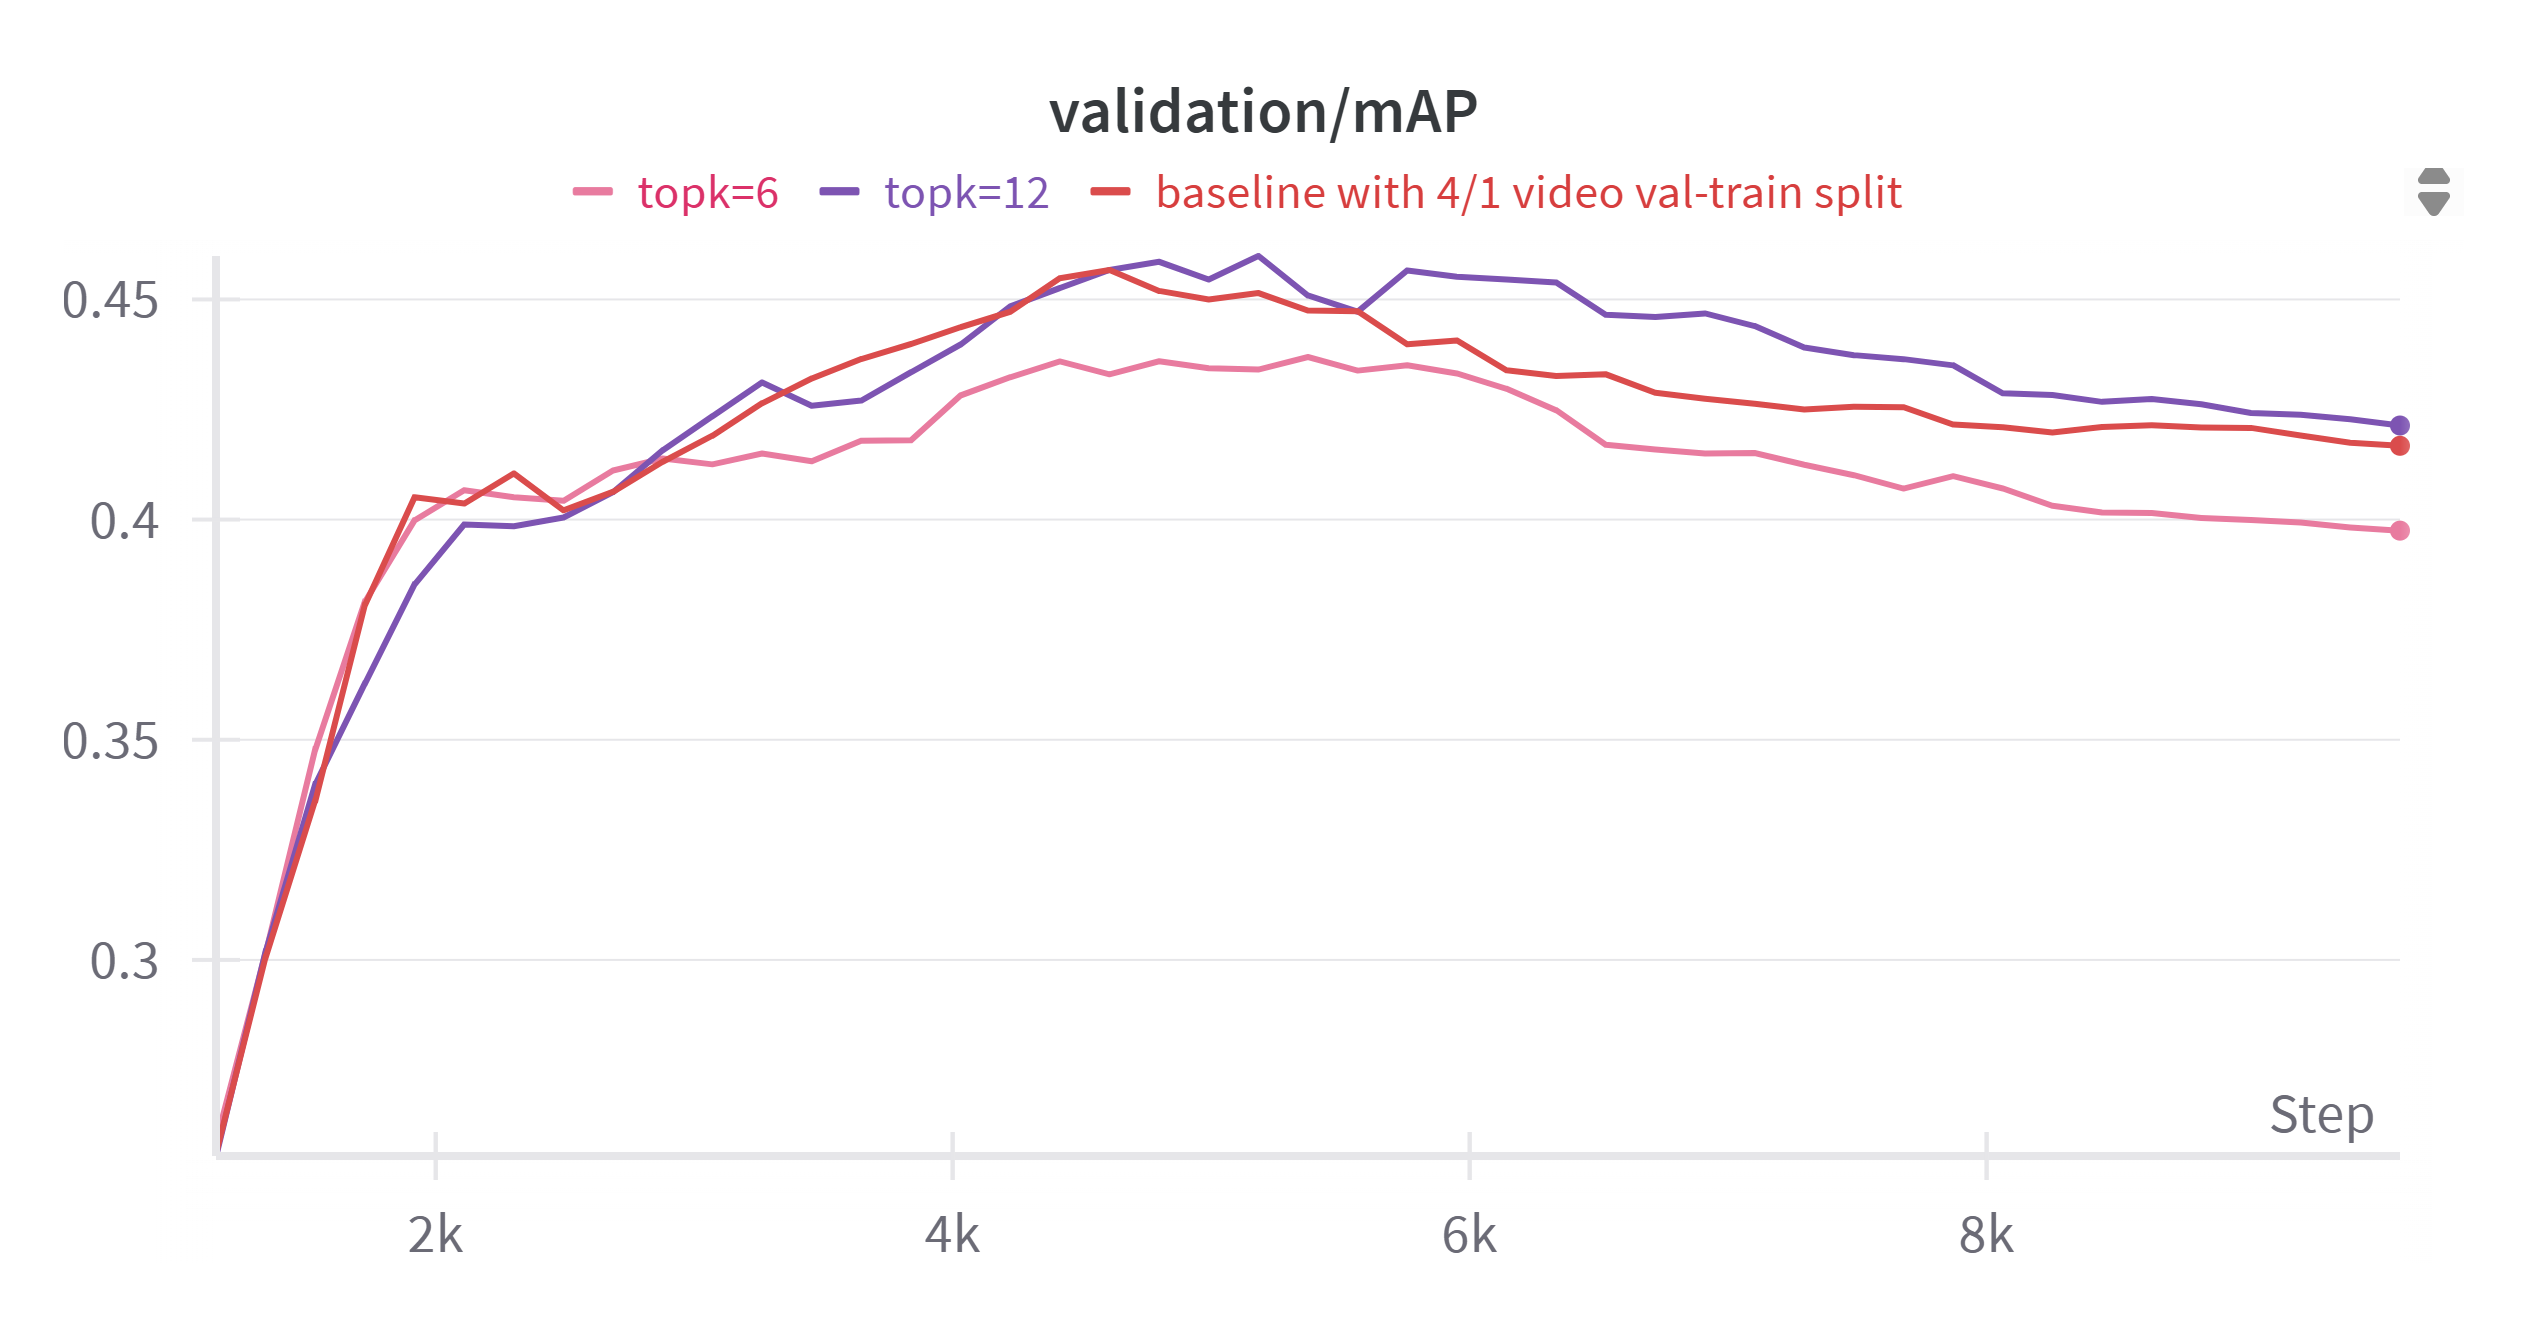
\includegraphics[width=0.75\linewidth]{figures/topk_classes.png}
    \caption{Results from different post-processing top \(k\) classes.}
    \label{fig:topk}
\end{figure}

Using a shorter stride for validation is a technique to increase training speed. In the case of the \acrshort{tdeed} implemented for SoccerNet, the testing phase is weighted more heavily than validation, as it is the submission to a challenge. This is an oversight; a run with \(STRIDE=1\) was run, but not completed in time for discussion. This oversight could be a hindrance to the direct comparison between the validation scores.\improvement{a run with stride=1 is run, but when will it complete? Late according to squeue --start --me}


% You suggest the "fine-grained nature of the action spotting task...is inherently well-suited to the \acrshort{tdeed} model's design." Could you expand on which specific design elements of \acrshort{tdeed} make it suitable for such tasks?

The temporal discriminability enhancer part of the \acrfull{tdeed} has specialized strategies and components designed to:
\begin{itemize}
    \item improve the distinction between similar actions
    \item improve token discrimination
    \item per frame predictions
\end{itemize}

The focus on enhancing temporal distinctions is one of the keys to success in tasks where small variations in timing or appearance can result in different categories. 

% How do the architectural differences between \acrshort{vms} (Mamba-\acrshort{s6}) and \acrshort{tdeed} relate to their observed performance characteristics in this experiment?

In contrast, Mamba's design captures long-range contexts and provides a broader understanding of the whole video. It is also meant to learn quicker with linear complexity and require less data. It is my theory that with a stronger post-processing pipeline, the \acrshort{map} advantage would be larger. 

% The \acrshort{tdeed} model used a specific train/validation split of 4 matches to 1. How comparable is this to the 80\%/20\% split used for the \acrshort{vms} model in terms of data representativeness or potential biases?

The validation set size of a single football game can be problematic. Football games can vary significantly due to teams, play styles, event frequency, and referee threshold for giving fouls, to name a few. There is a risk of bias from the distribution of actions within the validation game. If the validation game is "easy" or "hard", that would severely influence the validation score. A split of 80\% to 20\% validates on one game and trains on four in total. But when the game is split into 90 sections, which are randomly assigned to each category, the validation set is more robust. The result will be more transferable and generalizable. 

% Given the mixed results (VMS better on some metrics, T-DEED on another), what are the practical takeaways? When might one model be preferred over the other based on these findings?

\acrshort{vms} runs on any \acrshort{gpu}, but \acrshort{tdeed} needs a lot of memory and only runs on premium GPUs. If computational resources (especially GPU memory and type) are a limiting factor, \acrshort{vms} is the more practical choice. \acrshort{vms} has a simpler post-processing and a clearer GitHub explaining installation steps, which could be more straightforward to deploy. However, without obvious comparisons, it is hard to pick out clear advantages of one model over the other. 


% What are the main limitations of this first experiment that should be acknowledged in the discussion?

The most significant limitation is the absence of the test \acrshort{map}@50 score for the \acrshort{vms} model. This prevents a direct and complete comparison with \acrshort{tdeed} on this crucial metric, which is often considered the primary indicator of performance on unseen test data.

The \acrshort{tdeed} model was evaluated differently for validation and testing. The validation used a stride of two (halving temporal resolution) and lacked significant post-processing (like SNMS). The test evaluation used a smaller stride and included such post-processing. This inconsistency makes it difficult to:

\begin{itemize}
    \item Directly compare \acrshort{tdeed}'s validation \acrshort{map}@50 with its test \acrshort{map}@50.
    \item Fairly compare \acrshort{tdeed}'s validation \acrshort{map}@50 with \acrshort{vms}'s validation \acrshort{map}@50, as the evaluation conditions were not equivalent.
\end{itemize}

While \acrshort{tdeed}'s "four matches for training and one for validation" is an 80\%/20\% split, validating on a single match can be less representative and more prone to bias compared to an 80\%/20\% split.

Using "default hyperparameters from their original papers" might not be optimal for the specific SoccerNet-V2 dataset or the fine-grained action spotting task. These defaults might have been tuned for different datasets or tasks, potentially disadvantaging one or both models. This is tackled in \autoref{sec:experiment4}.



\section{Experiment 2: Compare runtime}
\label{sec:experiment2}

Wall-clock training time for each model on a Tesla A100 \acrshort{gpu} was recorded. Feature extraction was also timed, but separated from the time. \unsure{should I use identical epoch count and batch size?}
\todo{same number of epochs? Normalize for number of epochs?} 

\subsection{Setup}
\label{ssec:ex2_setup}

We know Mamba is faster than the Vit-based tdeed

MAMBA training took <3 Hours, but data extraction was slow. However also image extraction on tdeed was also slow. can say i ignore data preprocessing and just look at 


\section{Experiment 3: Feature increase}
\label{sec:experiment3}
To find out how much the size of the feature vector matters, a model with 1408 features and one with 3200 features is trained on the THUMOS-14 dataset.
InternVideo features have a size of 3200, and are the backbone of the \acrshort{sota} models on paperswithcode. The \acrshort{vms} models trained on Soccernet use 1408 features. Both models are trained with a Tesla V100-PCIE-32GB.


\subsection{Setup}
\label{ssec:ex3_setup}

To assess the effect of embedding size, two \acrshort{vms} instances were trained on THUMOS-14\cite{dataset:thumos}: one using 1,408-dimensional VideoMAE features and one using 3,200-dimensional InternVideo embeddings. All other settings, annotations, and hyperparameters remained identical.

The metrics are tracked using \acrlong{wandb} and console logs.
Both models were trained for 49 epochs on a Tesla V100-PCIE-32GB \acrshort{gpu}.

\subsection{Results}
\label{ssec:ex3_results}

\begin{figure}
    \centering
    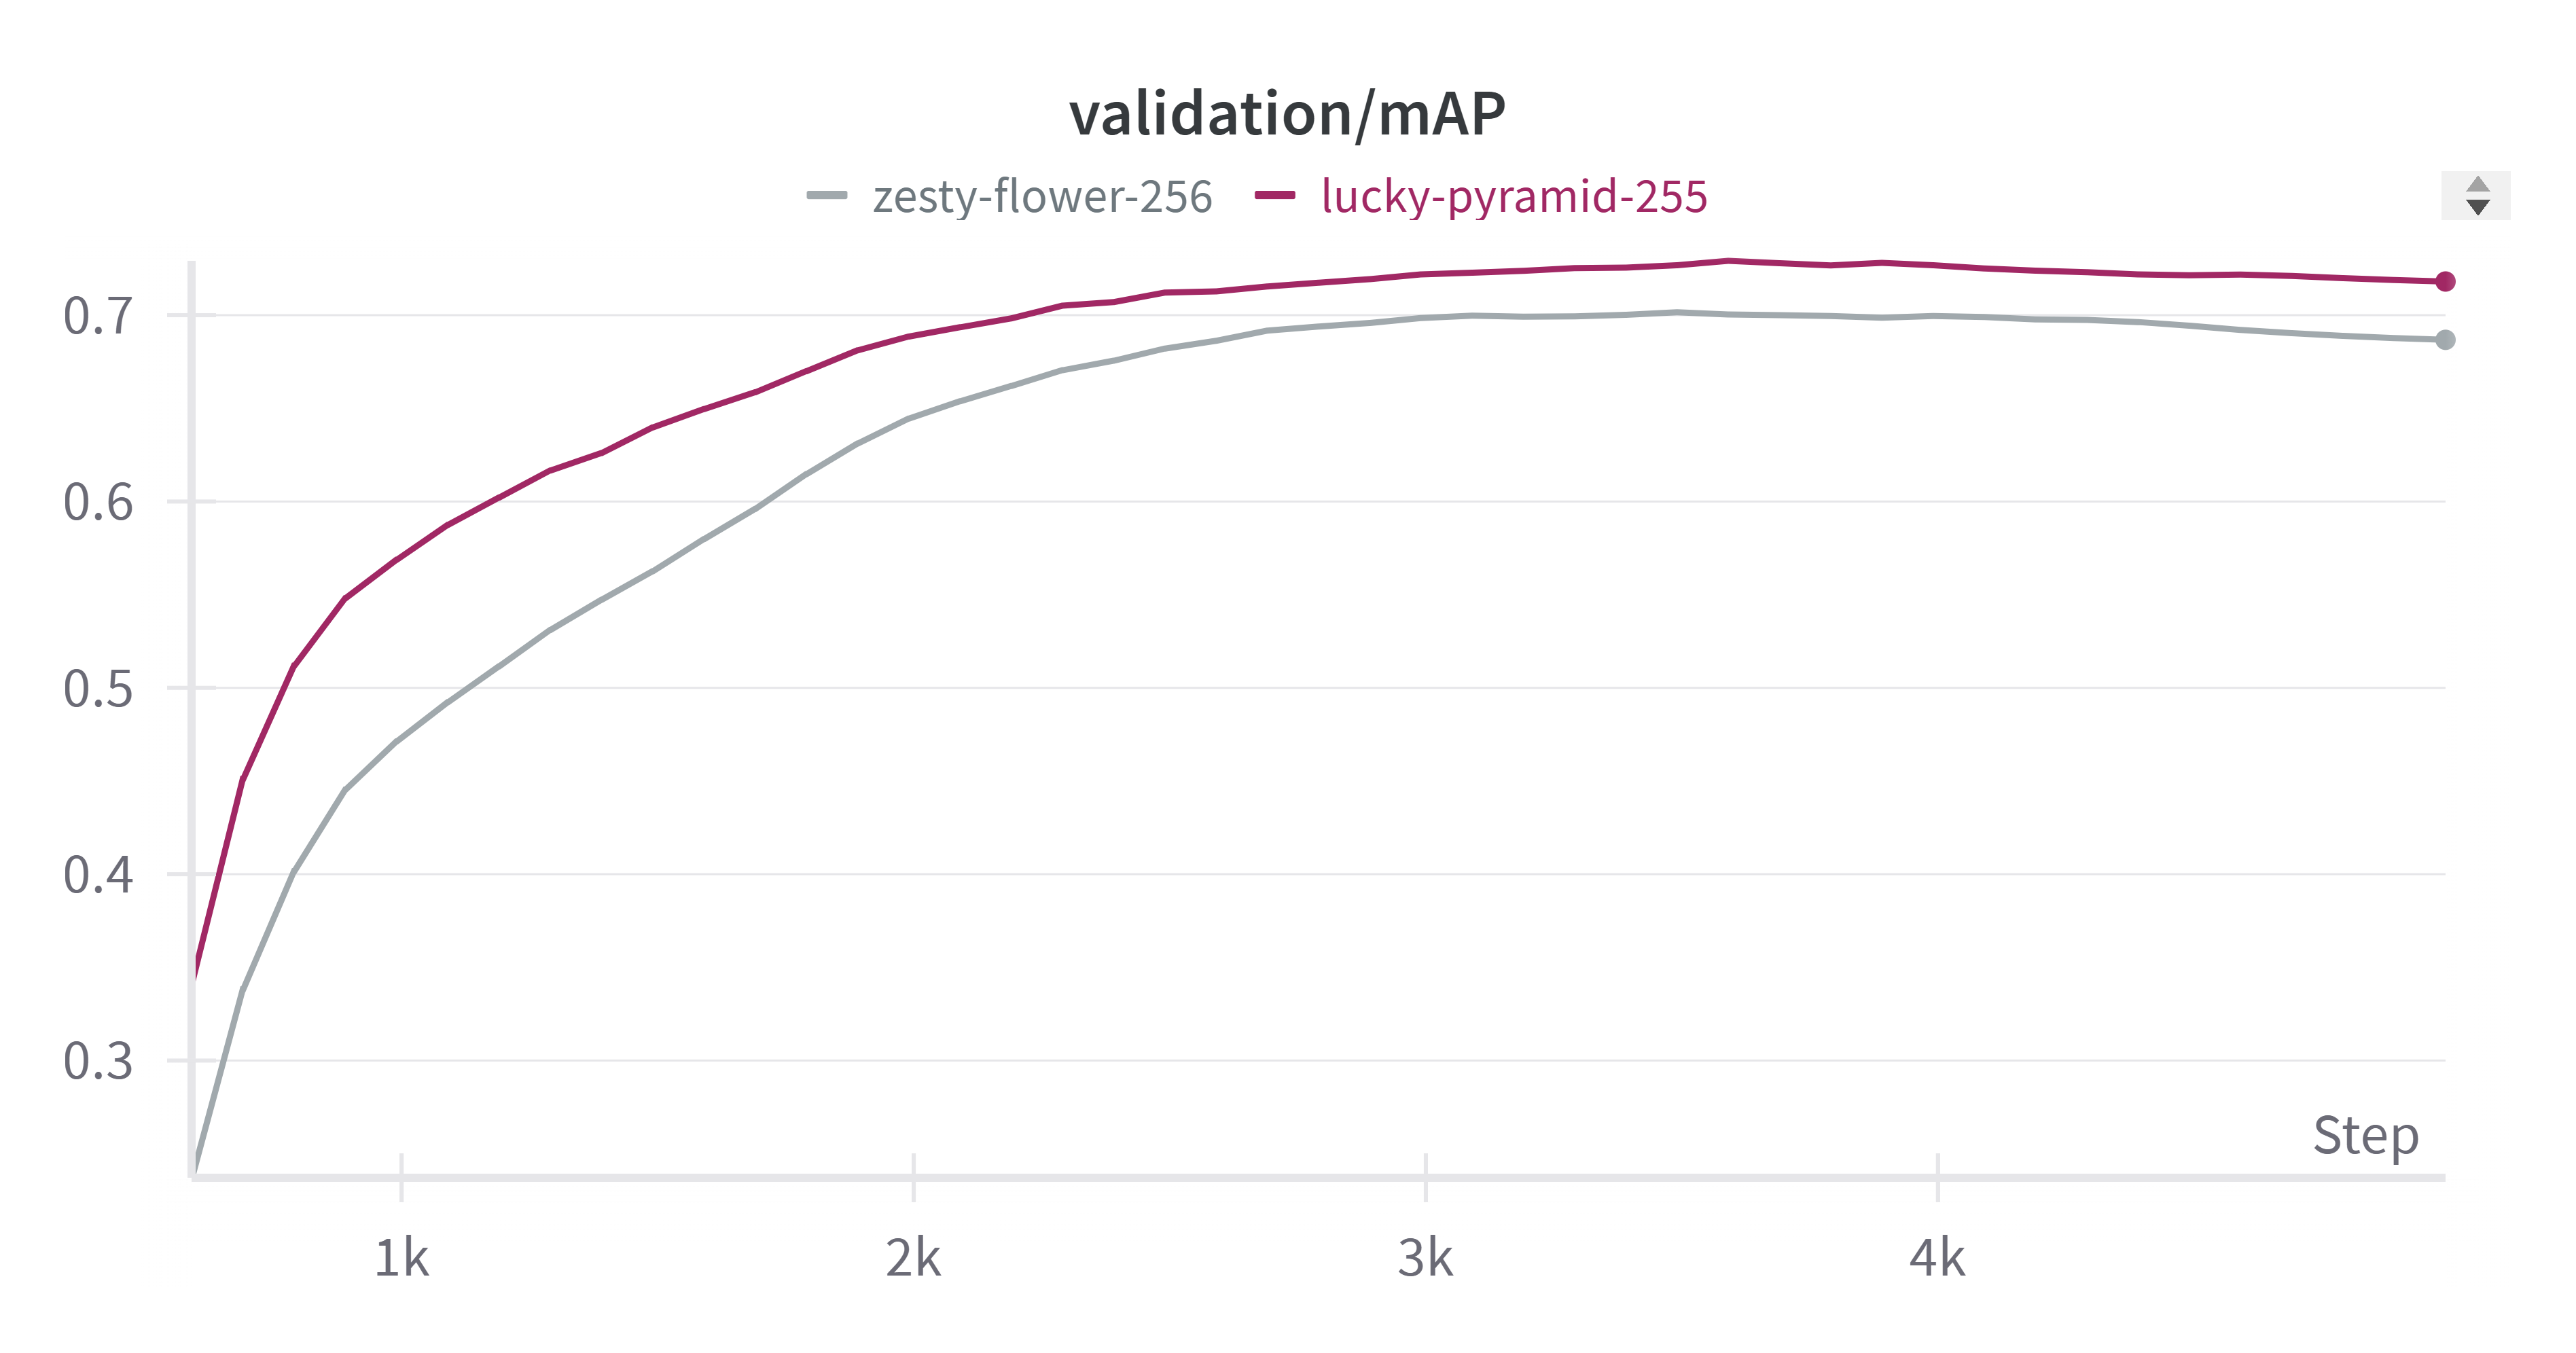
\includegraphics[width=0.75\linewidth]{figures/1408_3200_val.png}
    \caption{Validation per epoch for 3200 features (red) and 1408 features(grey). }
    \label{fig:ex3_val}
\end{figure}
The 1,408-dimensional model achieved a  \acrshort{map} of \(0.686\), while the 3,200-dimensional model reached a \acrshort{map} of \(0.718\) (a 3.2\% absolute gain). Training times were 1 h 15 min and 1 h 23 min respectively, which is an increase of \(\approx11\%\). \autoref{fig:ex3_val} 


\subsection{Discussion}
\label{ssec:ex3_discussion}

blessing of dimensionality. extra important in football or less important. More features => more probable for them to be linearly separable

favorable trade off(in time)

hyperparameters could favor the newer weights

both seem to hit a ceiling at epoch ~32


\section{Experiment 4: Hyperparameter optimization}
\label{sec:experiment4}

The fourth experiment is a hyperparameter optimization experiment.
The goal is to find the best hyperparameters for the \acrshort{vms} model on the SoccerNet dataset.

\subsection{Setup}
\label{ssec:ex4_setup}

\acrlong{wandb} is used to track the hyperparameters and the results for the \acrshort{vms} model trained on SoccerNet-V2 dataset with a 70 \(\%\)-30\(\%\) validation split. All 7 videos of the SoccerNet-V2-format is considered in this approach, including the train, the validation and the testing videos. A Bayesian optimization algorithm is used to find the best importance and correlation of the hyperparameters. The hyperparameters related to the dataset are the only ones modified. Full details about the hyperparameters can be found in \autoref{label:app_sweep}.

A total of 210 runs across three sweeps of 70 runs each were completed. Because of the fast convergence of \acrshort{vms}--models hyperparameter search was an efficient process. 


\subsection{Results}
\label{ssec:ex4_results}

\begin{figure}
    \centering
    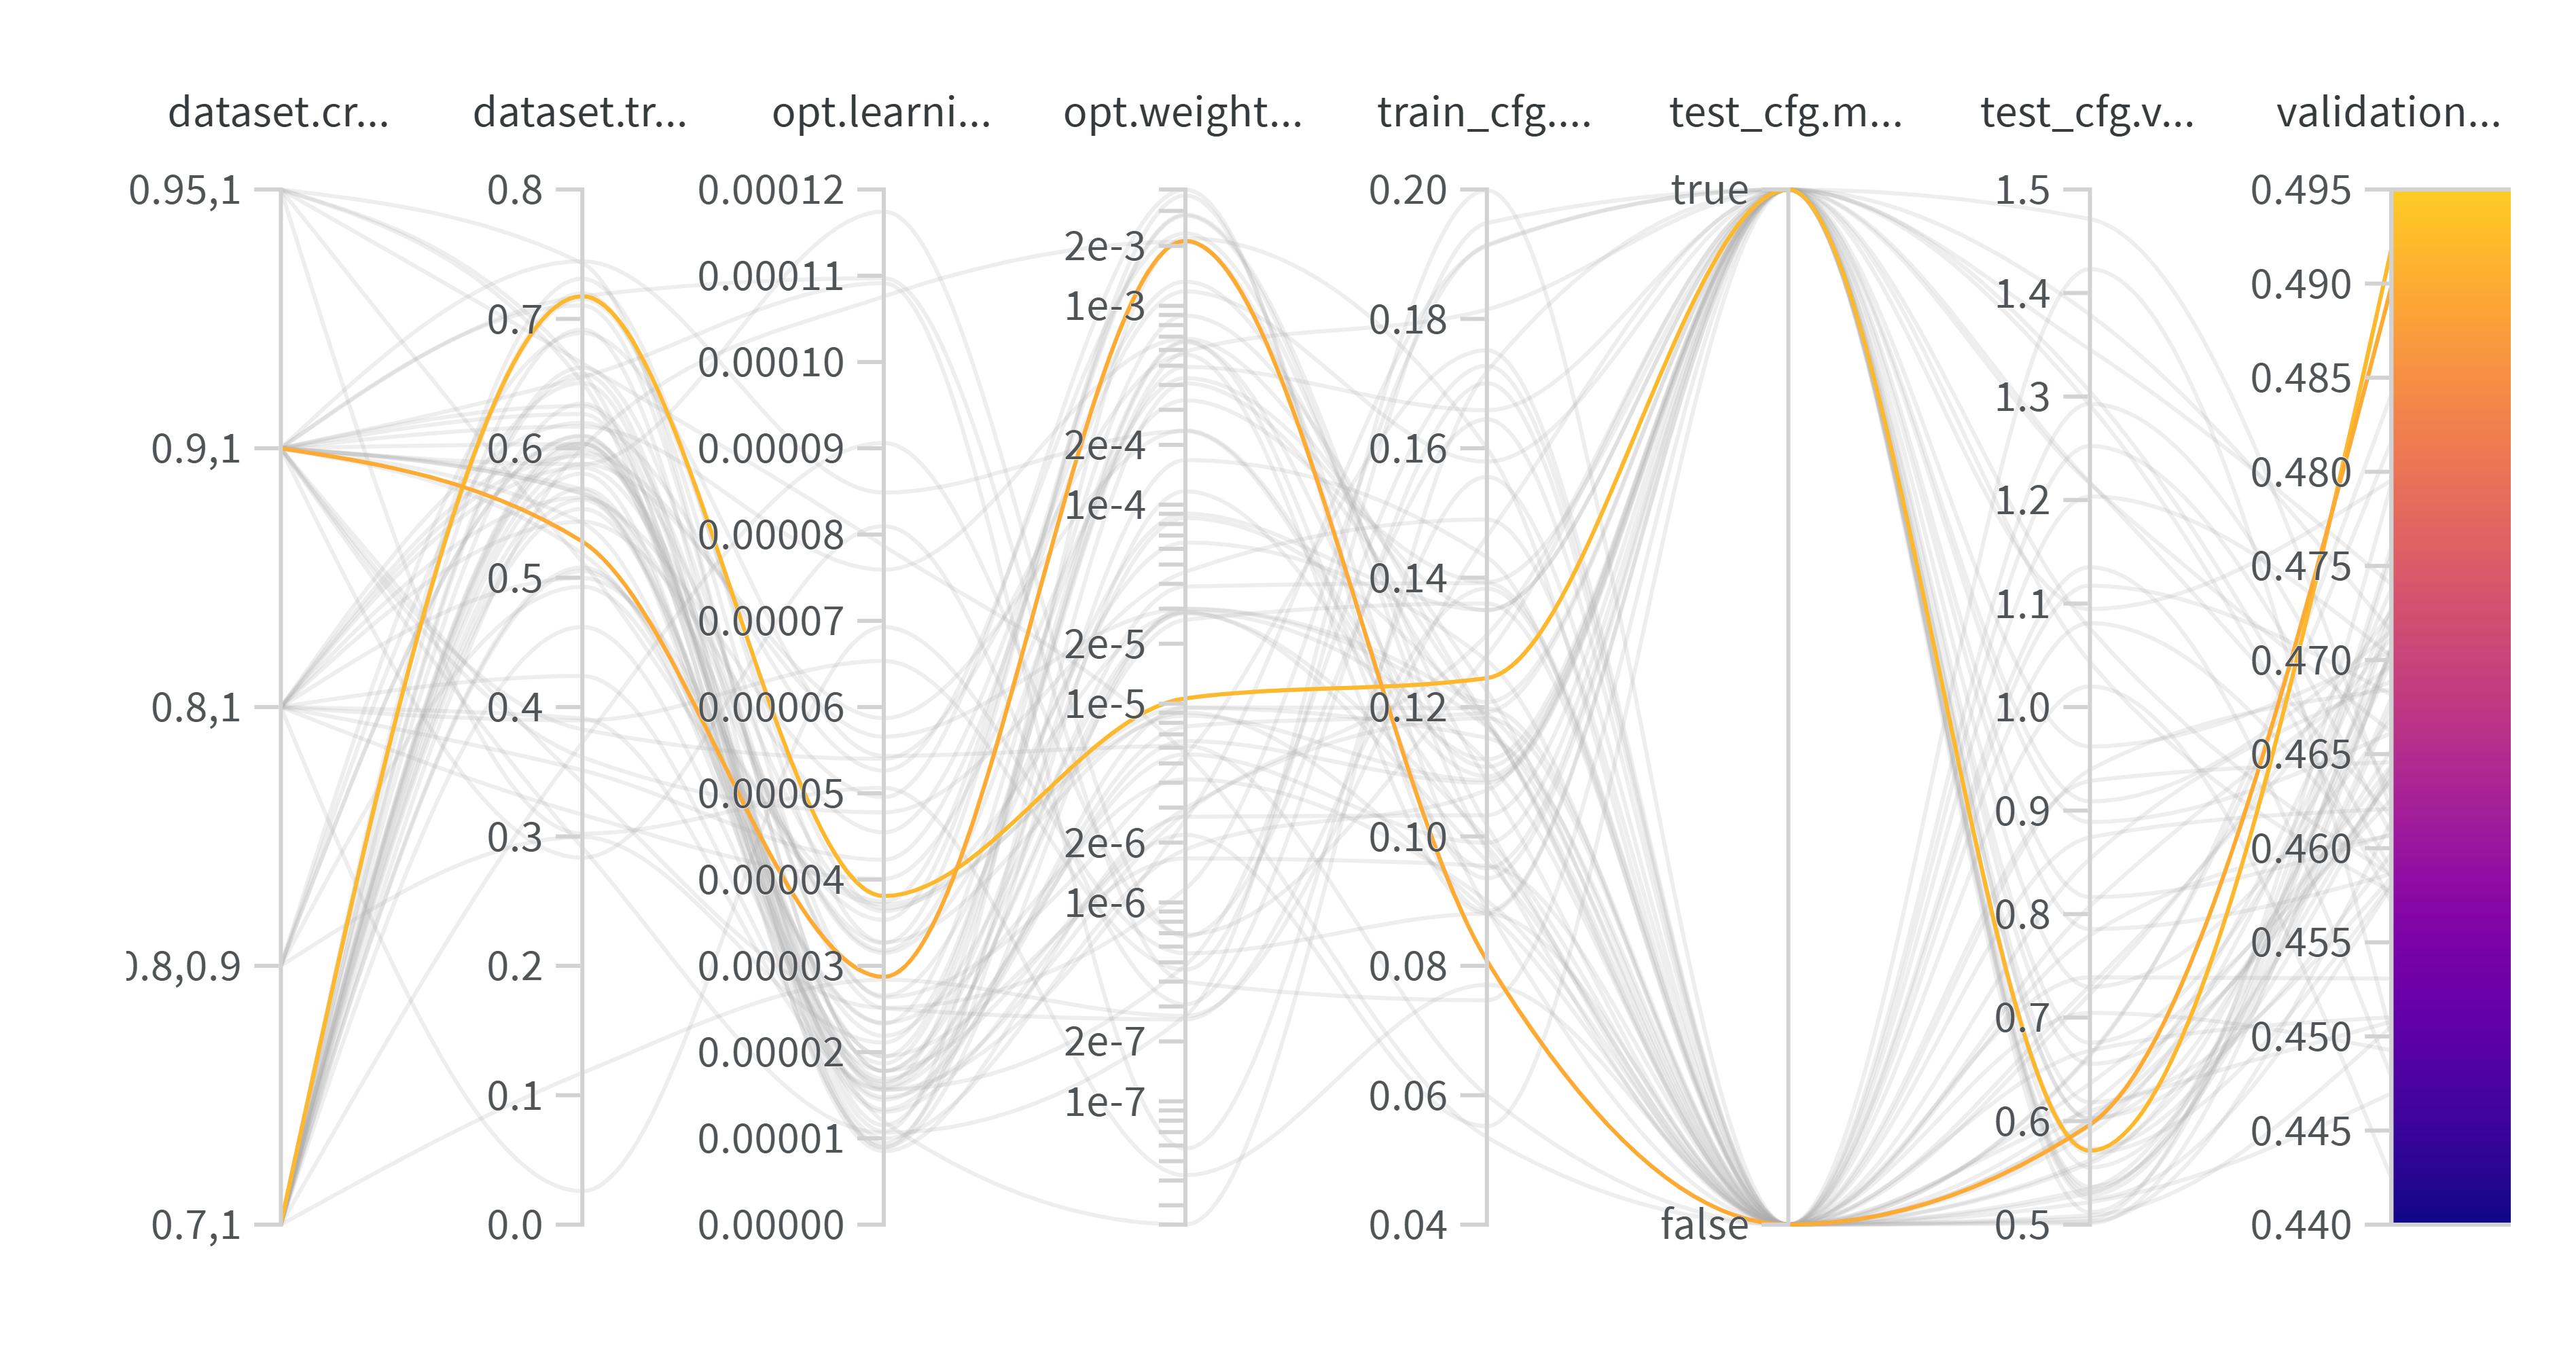
\includegraphics[width=1\linewidth]{figures/sweep_two_best.png}
    \caption{The hyperparameters of the two best results(yellow) compared to all runs (grey) in the thrid sweep. }
    \label{fig:sweep_best_two}
\end{figure}

The sweeps showed a slight improvement to the model. 

Trying to translate the sweep into a single better configration didn't prove useful, but some configurations performed exceptionally better than the rest. But these configurations that worked well, had quite different parameters and was hard to differ. As seen in \autoref{fig:sweep_best_two}, the hyperparameters of the best and second best run in the last sweep differed significantly in their hyperparameters. 

Interpreting the results to create a hyperparameter configuration, as explained in the \autoref{app:sweep_3} the resulting average \acrshort{map} was \(46.77\%\). 

\subsection{Discussion}
\label{ssec:ex4_discussion}

Multiple local optima in the search space. 

\improvement{image displaying local optima}

lower learning rate because football is homogeneous. many events are very similar
only tune dataset variables
negative/neutral results. why? i think its because features are trained to match the preprocessing timeline. some really good runs
something funny is up with the learning rate
overfit on 30 percent validation



\section{Experiment 5: T-DEED with and without joint training}
\subsection{Setup}
\label{ssec:ex5_setup}
\begin{figure}
    \centering
    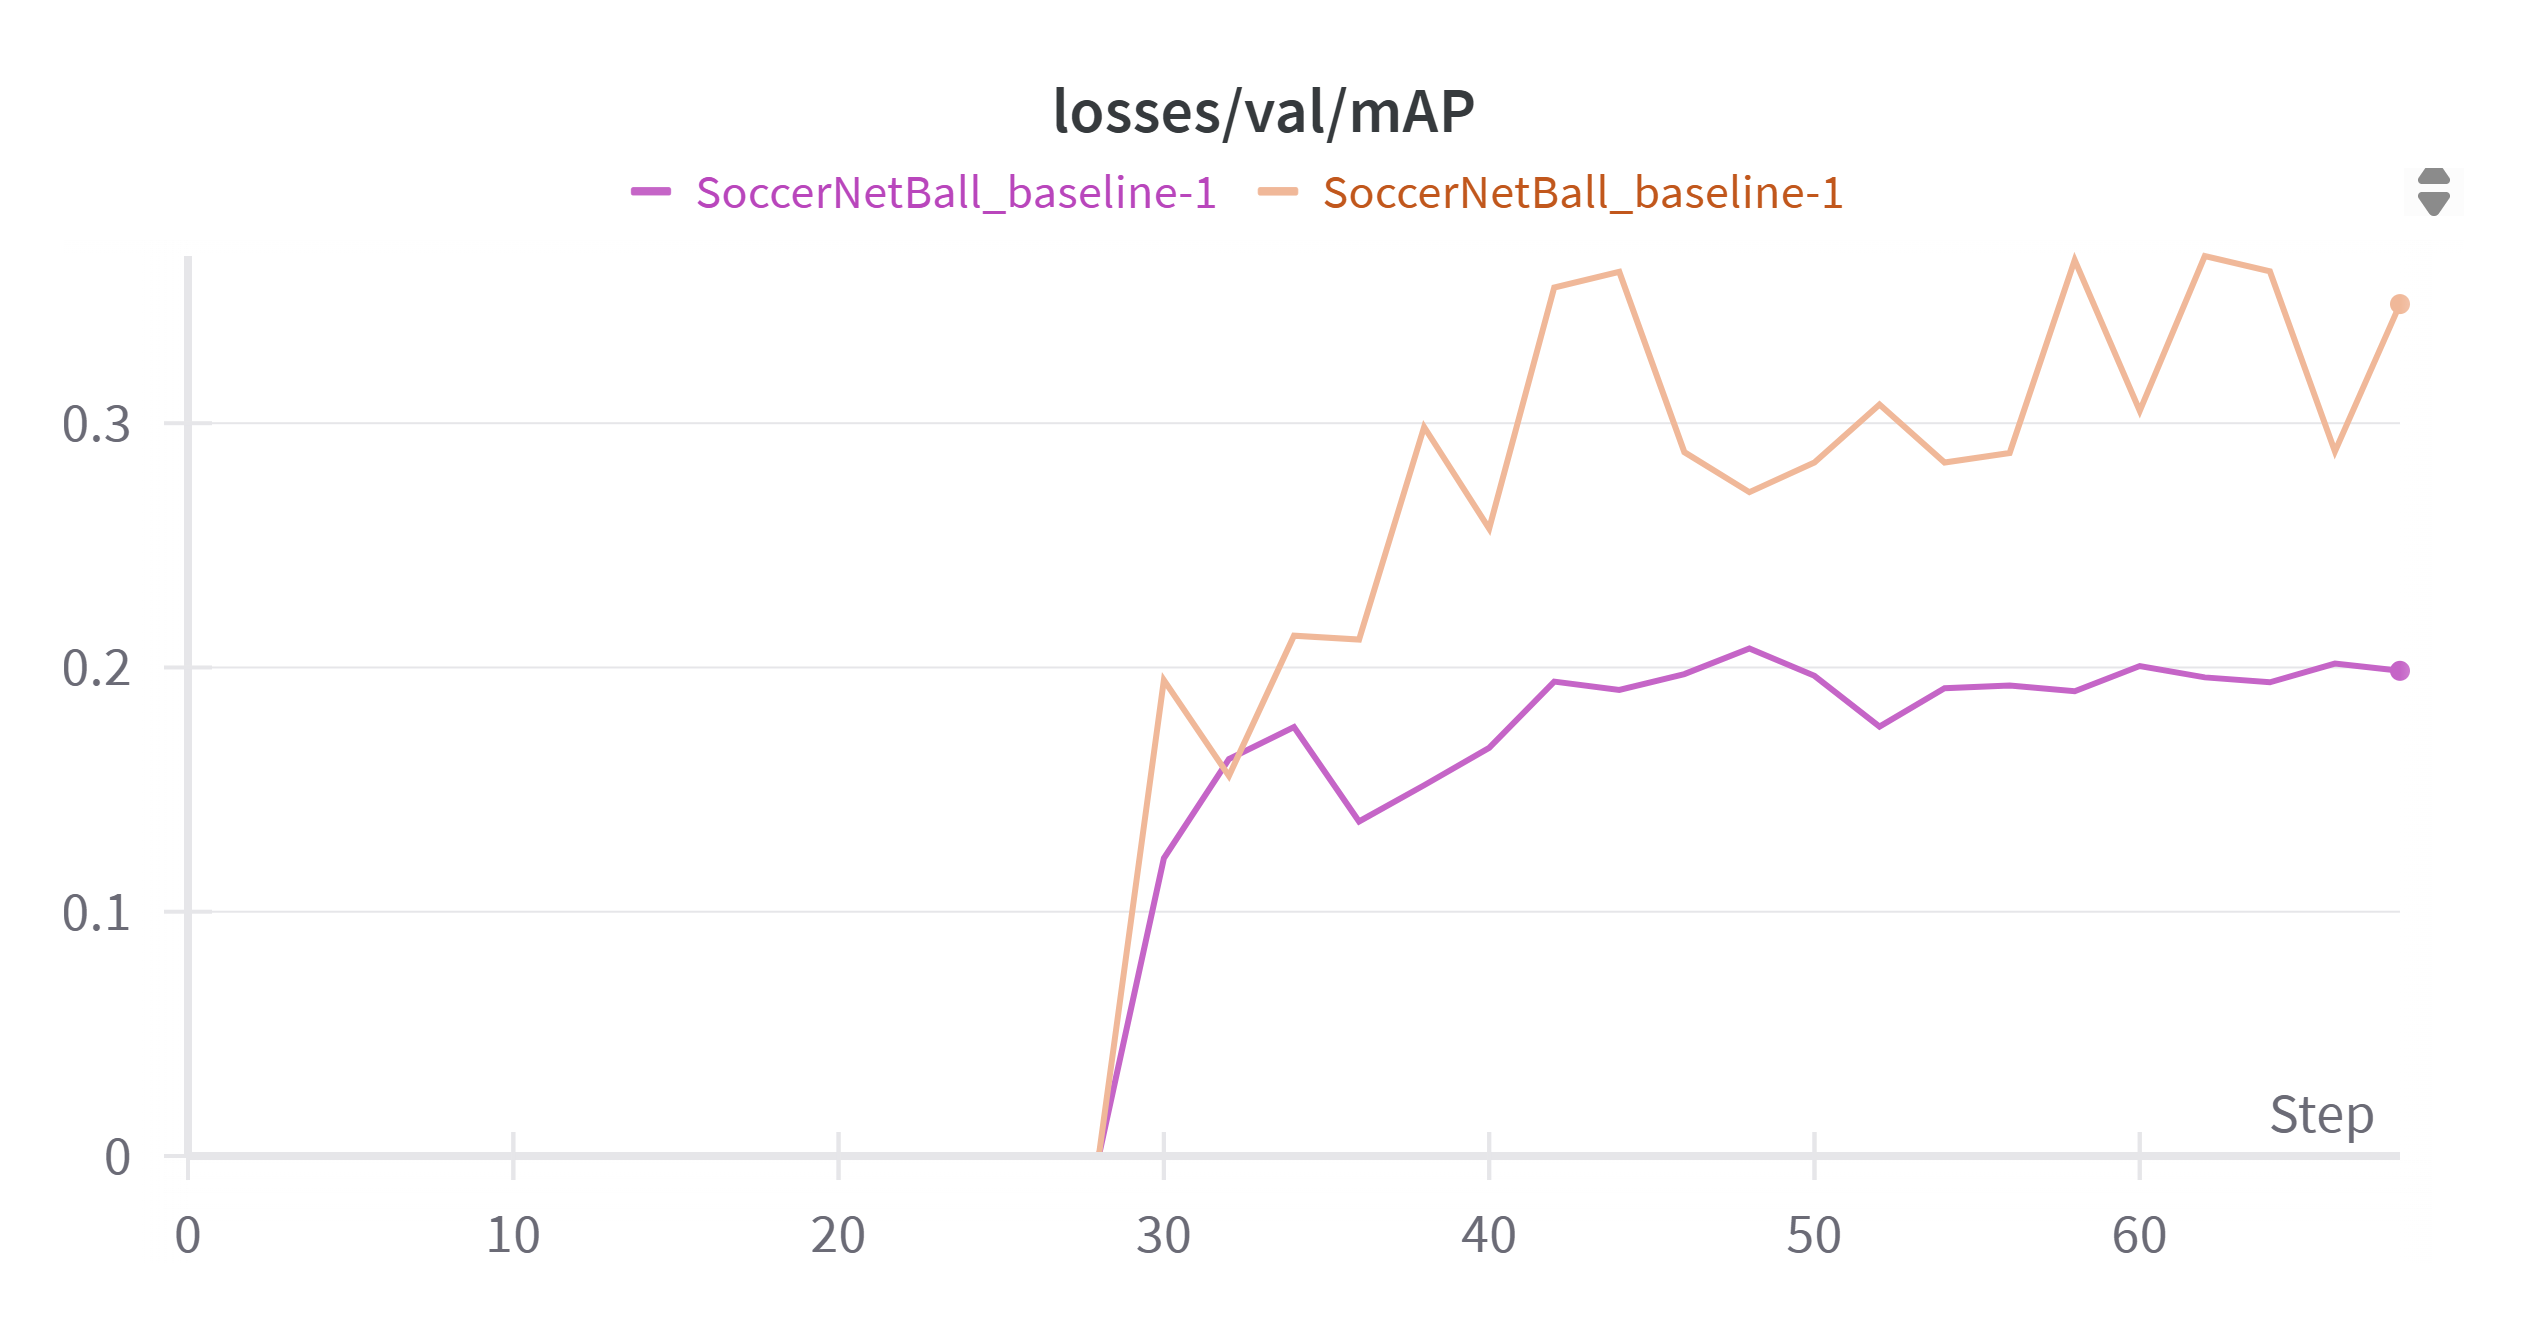
\includegraphics[width=0.75\linewidth]{figures/500_7_val_compare.png}
    \caption{Validation per epoch for the model trained with joint training (507 videos) in brown and the model trained without joint training (purple).}
    \label{fig:500_7_val_compare}
\end{figure}


\subsection{Results}
\label{ssec:ex5_results}


another experiment where I just run array jobs with different train/val splits

\subsection{Discussion}
\label{ssec:ex5_discussion}


\section{Summary}
vms runs on any GPU, but tdeed needs a lot of memory and only runs on premium GPUs.